\documentclass[11pt,a4paper]{article}

\usepackage{enumerate,graphicx}
% \usepackage{../durhampaper}
\usepackage{harvard}

\usepackage{enumitem}


\addtolength{\textwidth}{2.5cm}
\addtolength{\oddsidemargin}{-1.0cm}
\addtolength{\topmargin}{-1.5cm}
\addtolength{\textheight}{2.5cm}




\citationmode{abbr}
\bibliographystyle{agsm}

\title{Generative Models for Information Security: \\ Literature Review}
\author{{\bf Student:} John Jennings  \hspace{3mm} {\bf Supervisor:} Chris Willcocks}
\date{\today}




\begin{document}

 
\maketitle 

\section *{Problem Definition}
Generative models are important tools in machine learning, seeing recent success in a wide variety of applications, from synthesizing realistic images of human faces and house interiors, to transforming photos from summer to winter and night to day. Within the information security sector, they have been used for learning novel encryption schemes, modelling password distributions, and steganography techniques for hiding information within an image. This project will expand upon current research, and investigate the applications of generative models to lexical steganography.

\section *{Definition of Terms}
\begin{itemize}[leftmargin=0pt]
\item[] \textbf{Steganography} - The art of concealed communication, differing from cryptography in that the very existence of the message is secret. This is achieved by embedding the message into a seemingly innocuous \textbf{cover text} that can be sent to the intended recipient without arousing suspicion. 

\item[] \textbf{Stegotext} - The result of steganographically embedding a message into a particular cover text.

\item[] \textbf{Lexical Steganography} - A form of steganography concerned with embedding a message within written text through the use of redundancies in natural language e.g. word ordering, inclusion of adjectives or choice of synonyms.

\item[] \textbf{Generative Model} - A model that learns the underlying distribution of the training data in order to generate new samples from the same distribution.

\end{itemize}

\section *{Identified Issues and Themes}

\subsection *{Correspondence to Neural Machine Translation}
  While the concept of lexical steganography has existed for over a decade \cite{tlex}, there has been little research conducted in the area, with almost all existing solutions employing simple techniques based on synonym substitution \cite{universal}. A thorough search of the existing literature yielded only one paper that approached the problem from a machine learning perspective, Fang et al. \citeyear{lstm}, who proposed a solution for the weaker problem of \textit{cover generation} in which the user does not have control over the content of the cover text.\\
  As a result, we will instead draw inspiration from the more mature field of Neural Machine Translation (NMT). Intuitively, lexical steganography can be thought of as a translation task, in that we are transforming the input text from one form to another while preserving the meaning. Instead of translating English text into the equivalent German text, we are translating English text into an equivalent English text that embeds the secret message.
  

\subsection *{Modelling the Problem}

  From this perspective, we can view lexical steganography as a problem of learning a generative model over the distribution of cover texts, such that given a particular cover text, we can generate new texts that are semantically equivalent. Embedding the hidden message can then be achieved through a learned algorithm that maps a particular codeword to a particular equivalent text. Decoding the hidden message from the stegotext is then simply a case of undoing this mapping.\\

  \begin{figure}[htp]
    \centering
    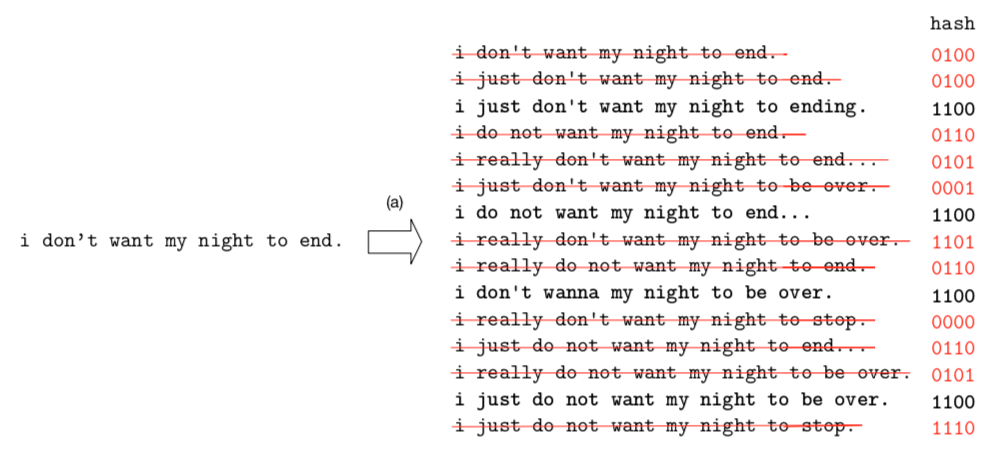
\includegraphics[width=0.9\textwidth]{mapping.png}
    \caption{An example of mapping semantically equivalent texts to codewords (Wilson et al. 2014). In this case, the codeword is determined by hashing the generated text.}
    \label{mapping}
  \end{figure}

  \nocite{covertweet1}

  \noindent We will now outline some examples of cutting-edge machine learning models and show how they can be modified for the purpose of lexical steganography.


  \subsubsection *{Autoencoder}
  In its simplest form, an autoencoder is a feed-forward neural network consisting of an input layer, a single hidden layer, and an output layer of the same size as the input. The model is then trained to output a reconstruction of the original input, thereby learning a latent representation of the input within the hidden layer. Modified versions of this relatively simple model have been successfully used for a number of applications, such as variable-rate image compression \cite{autoencimagecomp} and pretraining deep neural networks to have meaningful starting weights \cite{autoencstacking}. Compared to more traditional methods of unsupervised representation learning, such as principal component analysis, the autoencoder is shown to have a better expressive power, due to its ability to learn non-linear encodings \cite{goodfellow}.\\
  \indent One type of autoencoder that is of particular use for lexical steganography is the variational autoencoder (VAE), which learns to encode a training sample as a probability distribution over the latent space, instead of a single point. This is effective in generalizing the autoencoder to act as a generative model over the training distribution \cite{vae}. In the case of lexical steganography, a VAE could be trained on a set of cover texts such that at inference time, sampling from the distribution around a particular cover text will yield equivalent texts that can then each be mapped to a codeword.

  \begin{figure}[htp]
    \centering
    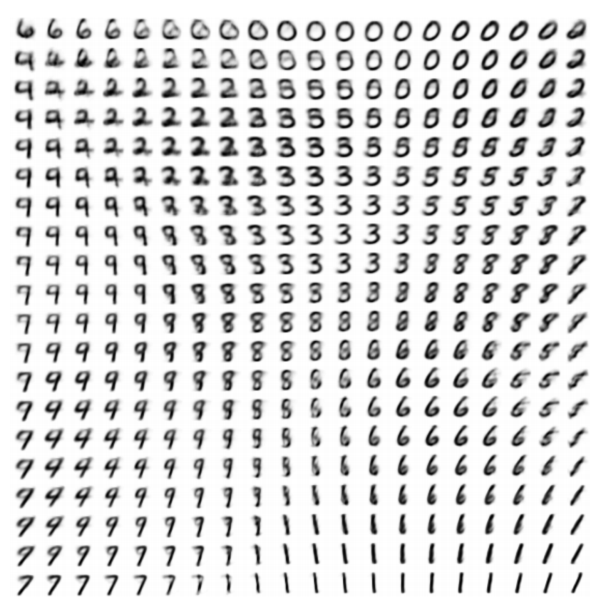
\includegraphics[width=0.6\textwidth]{mnist_manifold.png}
    \caption{A visualisation of the manifold learned by a VAE trained on the MNIST handwritten digits dataset (Kingma \& Welling 2013). }
    \label{manifold}
  \end{figure}

  \vspace{-5mm}
  \subsubsection *{Seq2Seq}
  In order to be able to apply an autoencoder-like architecture to lexical steganography, we must first deal with the issue of varying input and output size. Unlike models that operate over images, in which it is reasonably acceptable to crop and resize the input to a specific dimension, our model should be capable of handling text of an arbitrary length. Furthermore, it should not necessarily be true that the size of our input text matches the size of the output stegotext. For example, inputting ``Shall we go to the pub?'' as a cover text could result in an output stegotext of ``Do you want to go to the pub with me?''.\\
  \indent Fortunately, recent research in NMT provides a solution in the form of the Seq2Seq model \cite{seq2seq}. Similar to the autoencoder, it can be separated into an encoder RNN, which iterates over each token of the input sequence, modifying its internal state vector, and a decoder RNN, which takes the final hidden state of the encoder - the \textit{context vector} and outputs an arbitrary number of tokens in the target language. A novel aspect of this model is the inclusion of a hidden state within the decoder which provides an \textit{attention mechanism}, allowing the decoder to focus on different parts of the context vector as the output sequence progresses.\\
  \indent  This model can be easily trained as an autoencoder, with\nocite{seq2seqvae} Jang et al. 2018  providing a solution that modifies the Seq2Seq model to act as a variational autoencoder, showing improvements over a standard Seq2Seq autoencoder in the tasks of language modelling, missing word imputation, and paraphrase identification.

  \nocite{opennmt}
  \begin{figure}[htp]
    \centering
    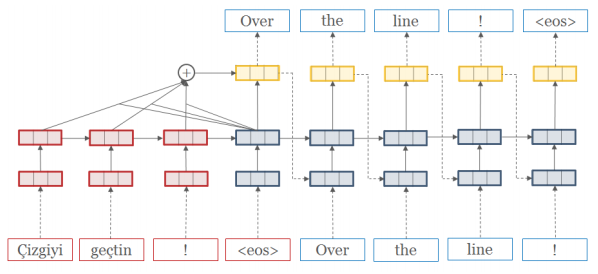
\includegraphics[width=0.6\textwidth]{nmt.png}
    \caption{A visualisation of a Seq2Seq model for translating Turkish to English (Klein et al. 2017). }
    \label{nmt}
  \end{figure}

  \subsubsection *{Generative Adversarial Network}
    An alternative model to the autoencoder is the Generative Adversarial Network (GAN), in which two networks, a generator and discriminator, are trained within a zero-sum game. The generator is given a random input and tasked with turning the input into a believable sample from the training set, while the discriminator is tasked with deciding if the given input is from the training set or the generator. As the discriminator learns to spot these `fake' generator samples, the generator will learn to make better fakes, effectively learning the latent space of the training steganography. \\
    \indent For the similar task of image steganography, GANs have been used to embed a secret message within an image in a content-adaptive manner \cite{gan2}, although these systems do not yet give better performance than purpose-built algorithms such as S-UNIWARD \cite{suniward}. Regarding lexical steganography, the effectiveness of a GAN is limited by the discrete nature of the generator's output. This prevents the gradient from propagating smoothly from the discriminator to the generator. \\
    \indent Yu et al. 2017 propose a solution to this problem in the form of seqGAN \nocite{seqgan}, which models the generator as a stochastic policy in reinforcement learning. The reward can be determined from the discriminator output, which is then backpropagated through the generator using the REINFORCE algorithm and a Monte Carlo search to determine the reward for incomplete sequences.


% \subsection *{Additional tuning}
%   word embeddings
%   skip connections
%   dropout

% \subsection *{Loss Function}
%   nll vs bleu

\section *{Proposed Direction of the Project}
  
  \subsection *{Dataset}
    Our model will be trained on a corpus of English-language posts from Twitter. This choice of dataset comes with a number of advantages, most notably that many previous lexical steganography systems, such as CoverTweet \cite{covertweet1}, are designed to work within the domain of Twitter, allowing for our system to be easily evaluated against existing methods. Furthermore, the casual context of Twitter allows for a greater steganographic capacity in the generated text. That is, misspellings and `interesting' grammatical choices are more acceptable in a tweet than in a Wikipedia article or news report. This increases the number of equivalent texts that can be derived from a particular cover text and in turn allows for more information to be embedded.
    % we basically just need a lot of english text, no need for labels etc
% lots of choice 
% everybody uses twitter for good reason
%   pretty standard form compared to prose
%   character limit <- good since RNNs tend to struggle on longer sequences
%   lots of data available
%   can compare against existing solutions
%   misspellings + slang -> more synonyms
%   has an immediate use case

  \subsection *{Proposed Model}
    Our proposed model will consist of an encoder, a decoder and a discriminator for adversarial training.
    The encoder (Fig. \ref{encoder}) is based on a Seq2Seq autoencoder with the addition of a payload vector that is present at every stage of the encoding process. This model could also be extended to act as a VAE as per Jang et al. 2018. The goal of the encoder is to output a sequence that is similar to the input sequence, can be decoded to reveal the payload, and cannot be detected as containing an embedded payload. \\
    \indent The goal of similarity between cover and stegotext can be measured by a loss function that compares the two. This could simply be their cross-entropy, or a purpose-built measure such as their expected BLEU score \cite{bleu}. To satisfy the remaining two goals, it is necessary to train a decoder  (Fig. \ref{decoder}) that takes the stegotext and extracts the payload, and a discriminator (Fig. \ref{discriminator})  that is given two sequences as input and must decide which sequence is the cover and which is the stegotext. 
    \begin{figure}[htp]
      \centering
      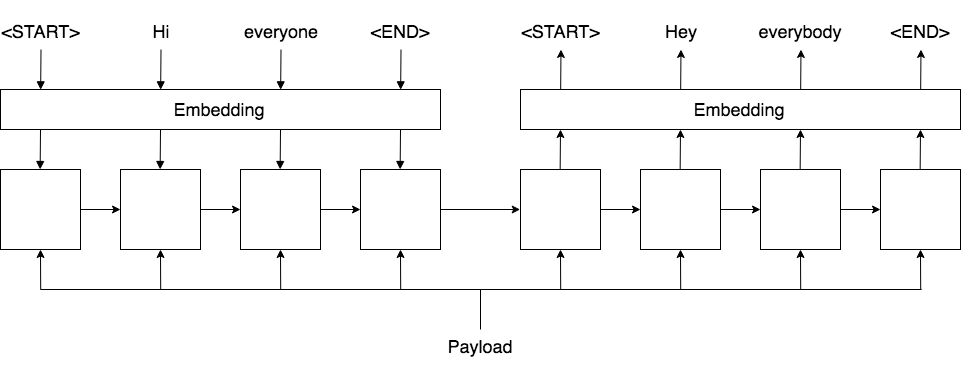
\includegraphics[width=0.9\textwidth]{encoder.png}
      \caption{A visualisation of the proposed encoder}
      \label{encoder}
    \end{figure}
    \begin{figure}[htp]{}
      \centering
      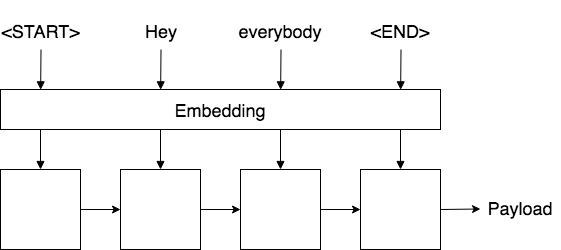
\includegraphics[width=0.6\textwidth]{decoder.png}
      \caption{A visualisation of the proposed decoder}
      \label{decoder}
    \end{figure}
    \begin{figure}[htp]
      \centering
      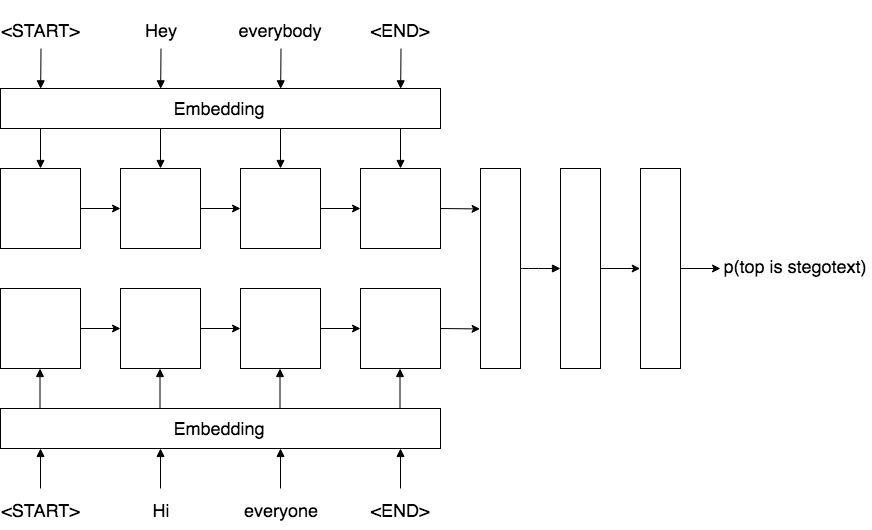
\includegraphics[width=0.9\textwidth]{discriminator.png}
      \caption{A visualisation of the proposed discriminator. }
      \label{discriminator}
    \end{figure}

\bigskip

\clearpage

\bibliography{../bib}
\end{document} 